\section{MTCNN Face Detection}
\label{MTCNN}
Bei Multi-task Cascaded Convolutional Neuronal Network (MTCNN) handelt es sich um ein Verfahren dass bei der Detektion von Gesichtern auch deren Ausrichtung berücksichtigt, um bessere Ergebnis zu erzielen.
\subsection{Constrained Local Neural Fields (CLNF)}
Dabei handelt es sich um einen Gesichtsdetektor. Für die Detektion wird für jedes Merkmal ein eigener Detektor auf einem Bildbereich angewendet und eine eigene Wahrscheinlichkeitskarte erstellt.\\
Als nächster Schritt wird das Ergebnissen der Detektoren mit eine Karte der Position aller Landmarks, mit ihrer Abweichung, kombiniert um somit die beste Position der Landmarks zu erhalten auf Bezug des Farbverlaufes und relativ zu den anderen Landmarks.
\cite{CLNF}
\subsection{Patch Experts}
Eine Bewertung, wie wahrscheinlich ein Landmark an einer bestimmten Position im Bild dargestellt ist. Dazu wird ein Bereich um die Position ausgewertet.
\cite{CLNF}
\subsection{Anforderungen}
Sein Einsatzgebiet ist die Vorverarbeitung eines Frames für die spätere Auswertung. Somit soll dieser Schritt von einem möglichst robusten Verfahren zur Detektion von Gesichtern durchgeführt werden.\\
Dabei kann auf einem hochauflösendem Bild mit verhältnismäßig kleinen, verschieden großen und weit verteilten Gesichtern gearbeitet werden.
\subsection{Die 3 Stufen der Verarbeitung}
Für die gute Detektionsqualität sorgt die dreistufige Verarbeitung mit verschiedenen CNN auf einer Bildpyramide. Bei der Bildpyramide handelt es sich um ein in verschiedenen Größen skaliertes Bild, damit der gesuchte Inhalt in der gewünschten Auflösung abgebildet ist, ohne dass etwas über den Inhalt zu wissen.\\
Dies ist von Vorteil, damit das CNN auf eine feste Größe von Gesichtern optimiert werden kann, um das Lernen, neben dem möglichen Farbverläufen, durch die Skalierung nicht zusätzlich zu erschweren und die CNN können auch auf ihre jeweilige Aufgabe besser optimiert werden können.
\begin{figure}
	\centering
	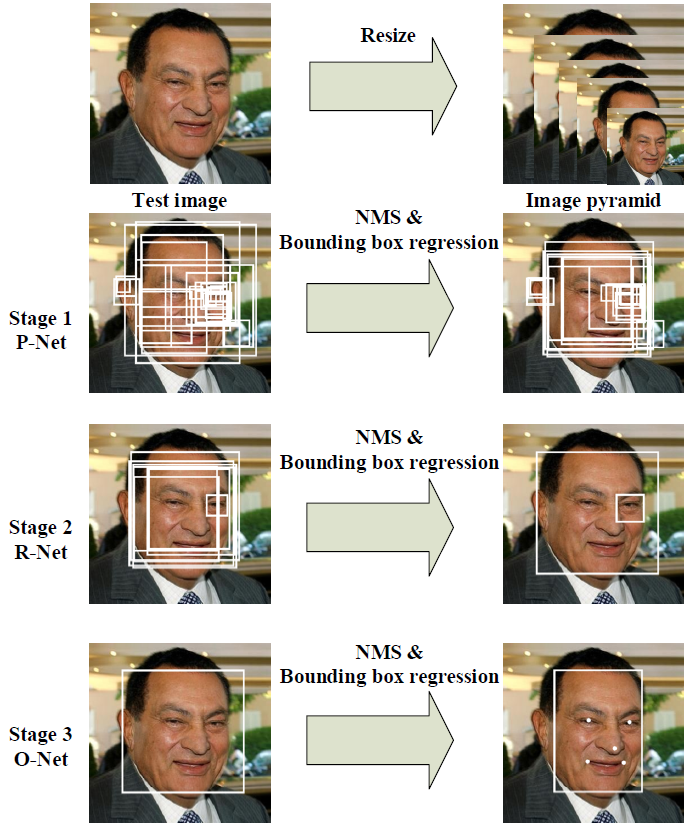
\includegraphics[width=0.5\linewidth]{img/MTCNN_Step}
	\caption{Darstellung des Funktionsablaufes von MTCNN\cite{MTCCN}}
	\label{img_MTCNN_Step}
\end{figure}
\subsubsection{Stufe 1}
Beim ersten Verarbeitungsschritt werden alle Bereiche eines Bilds gesucht, in denen möglicherweise ein Gesicht zu erkennen ist. Dazu wird für die Detektion ein CNN, dem sogenannten Proposal Network (P-Net), eingesetzt um alle möglichen Bounding-Boxen zu ermitteln in denen ein Gesicht zu sehen sein könnte. Diese Bounding-Boxen werden anschließend mit einem NMS ausgedünnt, um die am stärksten überlappenden Boxen zusammen zu fassen.
\subsubsection{Stufe 2}
Anschließend werden die möglichen Bereiche mittels eines weiten CNN analysiert, damit alle Nicht-Gesichtsbereiche erkannt und entfernt werden können.\\
Dies wird von dem Refine Network (R-Net) übernommen und anschließend die möglichen Bounding-Boxen mittels NMS weiter reduziert.
\subsubsection{Stufe 3}
Der letzte Schritt wird von einem deutlich genaueren CNN übernommen, um ein Gesicht zu detektieren, dem sogenannten Output Network (O-Net). Womit die resultierenden exakten Boxen und mit ihren jeweiligen 5 Landmarks ermittelt werden.
\subsection{Qualität}
MTCNN Face Detection ist bei der Zuverlässigkeit im Verglich zu anderen bekannten Verfahren überlegen, siehe \autoref{img_MTCNN_quality} und zudem Echtzeit fähig. Im Test-Datensatz sind auch Gesichtern mit einer Größe von $20\times 20$ Pixel enthalten und wurden erfolgreich erkannt.\\
Somit sind alle Anforderungen erfüllt um mit diesem Verfahren den vorhanden Frame für die nachfolgenden Berechnungen vorzubereiten.
\begin{figure}
	\centering
	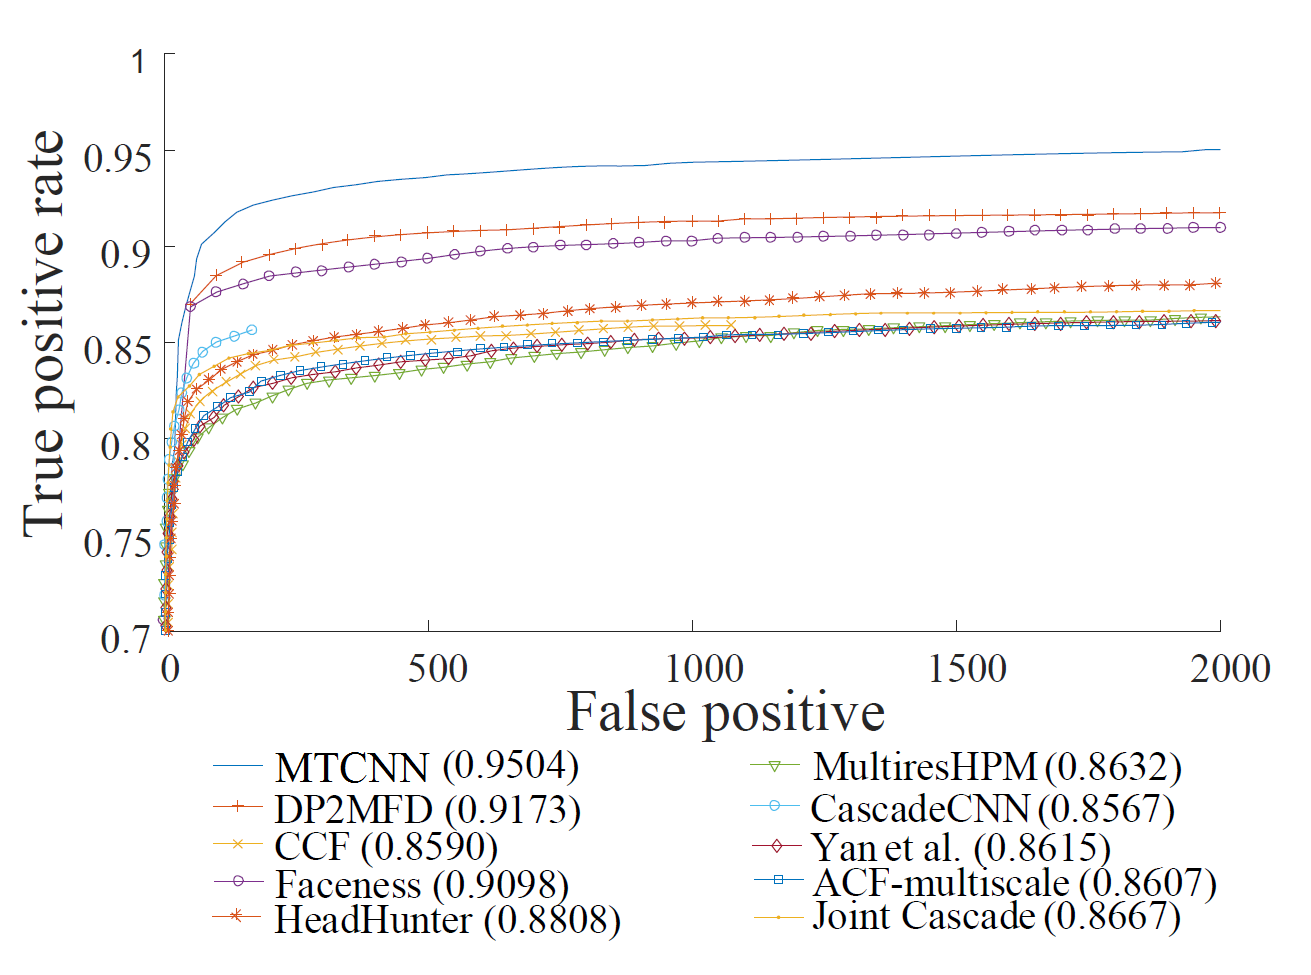
\includegraphics[width=0.5\linewidth]{img/MTCNN_quality}
	\caption{normale blaue Linie\cite{MTCCN}}
	\label{img_MTCNN_quality}
\end{figure}
%Joint Face Detection and Alignment using Multi-task Cascaded Convolutional Networks